\documentclass{bioinfo}

\usepackage{graphicx}
\usepackage{booktabs} % allows \toprule and other table formatting utilities
\usepackage{multirow} % merge cells vertically
\usepackage{colortbl} % Allows for alternate coloring the table
\usepackage[table]{xcolor} % U.a. allows for defining colors in HTML models
\usepackage{rotating} % Landscape orientation (used for tables)
\usepackage{color} % Only required for the TODO macro.

\usepackage[pdfborder={0 0 0}]{hyperref} % links, but no colored boxes
\usepackage{tabularx}
\usepackage{amssymb} % Symbols like checkmark
%\usepackage{lscape} % Landscape orientation (used for tables)


\hypersetup{breaklinks=true,
pagecolor=white,
colorlinks=false}
\urlstyle{rm} %so it doesn�t use a typewriter font for url�s.

% Allow line breaks in texttt
\newcommand{\origttfamily}{}% sollte noch nicht definiert sein!
\let\origttfamily=\ttfamily % alte Definition von \ttfamily sichern
\renewcommand{\ttfamily}{\origttfamily \hyphenchar\font=`\-}

\hyphenation{BioPAX BioCarta PaxTools SBML net-work net-works er-ro-neous-ly
      CellDesigner re-la-tion re-la-tion-ship re-ac-tion other-wise
      re-la-tions re-la-tion-ships re-ac-tions inter-action inter-actions re-search}

%%%%%%%%%%%%%%%%%%%%%%%%%%%%%%%%%%%%%%%%%%%%%%%%%%%%%%%%%%%%%%
% Useful macros:

%\newcommand{\TTra}{\textsuperscript{\tiny{}}}
\newcommand{\TODO}[1]{\textcolor{red}{\textbf{#1}}}

% B
\newcommand{\BiochemicalReaction}{\texttt{Bio\-chemical\-Reaction}}

% C
\newcommand{\Catalysis}{\texttt{Cata\-lysis}}
\newcommand{\ComplexAssembly}{\texttt{Complex\-Assembly}}
\newcommand{\Conversion}{\texttt{Conversion}}
\newcommand{\Control}{\texttt{Control}}
\newcommand{\Controller}{\texttt{Controller}}
\newcommand{\Controlled}{\texttt{Controlled}}
\newcommand{\ControlType}{\texttt{Control\-Type}}

% D
\newcommand{\Degradation}{\texttt{Degra\-dation}}
\newcommand{\DNAregion}{\texttt{DNAregion}}

% E
\newcommand{\Entity}{\texttt{Entity}}

% F
\newcommand{\functionTerm}{\texttt{function\-Term}}

% G
\newcommand{\GeneticInteraction}{\texttt{Genetic\-Interaction}}

% I
\newcommand{\inputP}{\texttt{input}}
\newcommand{\Interaction}{\texttt{Inter\-action}}

% M
\newcommand{\model}{\texttt{model}}
\newcommand{\Modulation}{\texttt{Modulation}}
\newcommand{\MolecularInteraction}{\texttt{Mo\-le\-cu\-lar\-In\-ter\-ac\-tion}}

% O
\newcommand{\outputP}{\texttt{output}}

% P
\newcommand{\Pathway}{\texttt{Pathway}}
\newcommand{\PhysicalEntity}{\texttt{Physical\-Entity}}

% Q
\newcommand{\qual}{\texttt{qual}}
\newcommand{\qualitativeModel}{\texttt{qualitative\-Model}}
\newcommand{\qualitativeSpecies}{\texttt{qualitative\-Species}}

% R
\newcommand{\reaction}{\texttt{reaction}}
\newcommand{\reactions}{\texttt{reactions}}
\newcommand{\RNAregion}{\texttt{RNAregion}}

% S
\newcommand{\sign}{\texttt{sign}}
\newcommand{\species}{\texttt{species}}
\newcommand{\Symbol}{\texttt{symbol}}

% T
\newcommand{\TemplateReactionRegulation}{\texttt{Template\-Reaction\-Regulation}}
\newcommand{\TemplateReaction}{\texttt{Template\-Reaction}}
\newcommand{\transition}{\texttt{transition}}
\newcommand{\transitions}{\texttt{transitions}}
\newcommand{\Transport}{\texttt{Transport}}
\newcommand{\TransportWithBiochemicalReaction}{\texttt{Transport\-With\-Biochemical\-Reaction}}

% End macros.
%%%%%%%%%%%%%%%%%%%%%%%%%%%%%%%%%%%%%%%%%%%%%%%%%%%%%%%%%%%%%%

\copyrightyear{2012}
\pubyear{2012}

\begin{document}

\firstpage{1}

\title[BioPAX to SBML qual]{Qualitative translation of relations from BioPAX to SBML qual}
\author[Finja B\"uchel \textit{et~al.}]{
Finja B\"uchel\,$^{1\,,}$\footnote{to whom correspondence should be
addressed}\,, Clemens Wrzodek\,$^1$,
Florian Mittag\,$^1$,
Andreas Dr\"ager\,$^1$,
Johannes Eichner\,$^1$,
Nicolas Rodriguez\,$^2$,
Nicolas Le Nov\`{e}re\,$^2$,
and Andreas~Zell\,$^1$}
\address{$^{1}$Center for Bioinformatics Tuebingen (ZBIT), University of Tuebingen, T\"ubingen, Germany
\\
$^{2}$Computational Systems Neurobiology Group, European Bioinformatics Institute, Hinxton, United~Kingdom
}

\history{Received on XXXXX; revised on XXXXX; accepted on XXXXX}

\editor{Associate Editor: XXXXXXX}

\maketitle

\begin{abstract}
\section{Motivation:}
The Biological Pathway Exchange Language (BioPAX) and the Systems Biology Markup Language (SBML) belong to the most popular modeling and data exchange languages in systems biology.
The focus of SBML is quantitative modeling and dynamic simulation of models, whereas the BioPAX specification concentrates mainly on visualization and qualitative analysis of pathway maps.
BioPAX describes reactions and relations.
In contrast, reactions are the only type of interaction in core SBML.
With the SBML Qualitative Models extension (\qual), it has recently also become possible to describe relations in SBML.
Before the \qual{} creation, relations could not be translated into SBML at all or were erroneously converted to reactions.
Until now, there exists no BioPAX to SBML converter that is fully capable of translating both reactions and relations.
\section{Results:}
The entire Nature Pathway Interaction Database (PID), which includes pathways from BioCarta, Reactome, and from the National Cancer Institute has been converted from BioPAX into SBML.
All available PID BioPAX pathway files (Level~2 and Level~3) have been translated into the SBML format (Level~3 Version~1) including both reactions and relations by using the new \qual{} extension package.
Additionally, we present the new webtool BioPAX2SBML, which can be used for further BioPAX to SBML conversions.
\section{Availability:}
BioPAX2SBML is freely available at \url{http://webservices.cs.uni-tuebingen.de/} and the complete collection of the PID models at \url{http://www.cogsys.cs.uni-tuebingen.de/downloads/Qualitative-Models/}.
%The complete collection of the PID models is freely available at \url{http://www.cogsys.cs.uni-tuebingen.de/downloads/Qualitative-Models/}and the webtool BioPAX2SBML at \url{http://webservices.cs.uni-tuebingen.de/}.
\section{Contact:}
%\href{finja.buechel@uni-tuebingen.de}{finja.buechel@uni-tuebingen.de}
\href{mailto:finja.buechel@uni-tuebingen.de}{finja.buechel@uni-tuebingen.de}
\end{abstract}




\section{Introduction}
The goal of systems biology is the model-driven understanding of biological and biochemical processes across all layers and various levels of detail.
The Biological Pathway Exchange Language (BioPAX) and the Systems Biology Markup Language (SBML) are common modeling languages that facilitate the exchange and storage of \emph{in-silico} models.
BioPAX can be used to describe the biological semantic of  metabolic, signaling, molecular, gene-regulatory and genetic interaction networks \citep{Demir2010}.
SBML describes the structure of models, and offers the possibility to include mathematical expressions \citep{Hucka2003}.
The SBML core specification defines reactions in detail but no other relationships between molecules.
%problem
Those relationships are denoted as \emph{relations} that specify enzyme-enzyme relations, protein-protein interactions, interactions of transcription factors and genes, protein-compound interaction, links to other pathways, etc.
Before the creation of the Qualitative Models extension for SBML (\qual, \citealp[see][]{QualSpecification}), it was not possible to define relations or to include reactions together with relations in one model.
%relevance
Furthermore, the combination or exchange of information between different databases is hardly feasible if one database uses the BioPAX format and the other one the SBML format.
%literature review
So far, there exist several visualization tools, such as Cytoscape \citep{Zinovyev2008, Smoot2011a} or CellDesigner \citep{Funahashi2007, Mi2011}, which can handle BioPAX and SBML by using plugins. But the combination of both formats or conversion of one format into the other is difficult even with these plugins.
Hence, converters are needed.

Today, there exist mainly converters from SBML to BioPAX like \emph{The System Biology Format Converter} \citep[see][]{SBFC}, but no converter for BioPAX to SBML that is capable of properly including relations.
Other research groups previously faced the same problem with incompatibilities between BioPAX and SBML.
To overcome the limitations of those file formats and to avoid the creation of pseudo-reactions or similar constructions, \citet{Ruebenacker2009} introduce an intermediate bridging format.
%
The need to combine both formats to use the knowledge from a multitude of databases in various applications becomes more and more urgent.

% what we did
% necessary to mention why we use PID?
In this paper we present a webtool for the translation from BioPAX into SBML format. We demonstrate its functionality by converting the whole Nature Pathway Interaction Database (PID, \citet{Schaefer2009} from BioPAX Level~2 and Level~3 formats to the SBML format, including the \qual{} extension.
%The translated files are freely available at \url{http://www.cogsys.cs.uni-tuebingen.de/downloads/Qualitative-Models/}.
% what we find out?
% what do the results mean (why are they significant?)




\begin{methods}
\section{Material and Methods}
\subsection{SBML and the Qualitative Models extension}
%%%%%%%%% SBML
The SBML Level~3 Version~1 core specification defines a special XML dialect to describe quantitative models.
The most important classes are \species{}, describing reactive species, and \reactions{}, which interconnect \species{} elements.
A \species{} element can be further specified with the aid of MIRIAM annotations \citep{Novere2005}.
The SBML core specification provides no possibility to define other relationships than concrete quantitative reactions.

%%%%%%%%% SBML qual
The SBML Qualitative Models extension (\qual) introduces qualitative elements, such as \qualitativeSpecies{} and \transition, providing the necessary means to describe relationships that can not be described by reactions, for instance, enzyme-enzyme relations or interactions of transcription factors and genes \citep{QualSpecification}.
%%%%%%%%%%%%% replaced version
% Although, technically, those processes are chemical reactions, too, it can
% often be far more useful to represent them by logical states and transitions.
%Instead of concentration levels, that are transformed continuously via reactions, \qualitativeSpecies{} have discrete states that are changed using {\transition}s.
%These {\transition}s consist of \inputP{} and \outputP{} elements.
%The \sign{} attribute of the \inputP{} elements describes wether the relationship between the \inputP{} and \outputP{} elements is \emph{positive}, \emph{negative}, \emph{dual}, or \emph{unknown}.
%\emph{Dual} means that the transition can operate both activating (\emph{positive}) and inhibiting (\emph{negative}).
%In contrast, \emph{unknown} is assigned to the \inputP{} if the transition effect is not further specified.
%If, in a qualitative model, protein A inhibits protein B, this would be represented as a \transition{} with \inputP{} A, whose \sign{} attribute is \emph{negative} and \outputP{} B.
Instead of the quantities associated to \species, which are affected by reactions, \qualitativeSpecies{} exhibit discrete states, representing their activities that are changed using transitions.
These transitions are linked to \inputP{} and \outputP{} elements.
The \sign{} attribute of the \inputP{} elements describes whether the relationship between the \inputP{} and \outputP{} elements is \emph{positive}, \emph{negative}, \emph{dual}, or \emph{unknown}.
\emph{Dual} means that the transition can operate both activating (\emph{positive}) and inhibiting (\emph{negative}).
In contrast, \emph{unknown} is assigned to the \inputP{} if the transition effect is not further specified.
If, in a qualitative model, the activity of protein A inhibits the activity of protein B, this would be represented as a transition with an input A, whose \sign{} attribute is \emph{negative}, and an output B.


\subsection{The BioPAX specification}
The Biology Pathway Exchange Language (BioPAX) is an OWL (Web Ontology Language) dialect based on RDF.
There is one superclass called \Entity{} that is extended by all other BioPAX classes.
Two main classes are distinguished: \PhysicalEntity{} and \Interaction.
\PhysicalEntity{} describes molecules, such as proteins, complexes, small molecules, DNA, or RNA, whereas \Interaction{} defines reactions and relations between \PhysicalEntity{} classes.
\Interaction{} is split into \Control{} and \Conversion{}, which can be separated into the subclasses \Catalysis, \Modulation, \TemplateReactionRegulation, \TemplateReaction, \GeneticInteraction, \MolecularInteraction,
\Transport, \BiochemicalReaction, \TransportWithBiochemicalReaction, \Degradation{}, and \ComplexAssembly.

BioPAX is released level-wise with the current level being Level~3.
Level~1 is exclusively able to describe metabolic interactions, whereas Level~2 supports signaling pathways and molecular interactions.
In addition to Level~2, gene-regulatory networks and genetic interactions can be described with Level~3.
For this purpose the \Control{} subclass \TemplateReactionRegulation, the \Conversion{} subclass \Degradation{}, \TemplateReaction, \GeneticInteraction, and \MolecularInteraction{} have been added.
Furthermore, \PhysicalEntity{} is now able to define \DNAregion{} and \RNAregion.
Level~3 is not downwards compatible with Level~2, but Level~2 is downwards compatible with Level~1 \citep{Demir2010}.
The BioPAX specification of Level~2 denotes all classes in lower case typewriter font and the specification of Level~3 denotes them in upper case typewriter font. For better readability of this paper, all BioPAX element names begin with capital letters and refer to Level~2 and 3. In contrast, SBML classes are written in lower case.




\subsection{Conversion of BioPAX to SBML \qual}\label{subsec:BioPAX}
%%%%%%%%%%%%%%%%%%%%%%%%%%%%%%%%%%%%%%%%%%%%%%%%%%%%%%%%%%%%%%%%%%%%%%%%%%%%%%%%%%%%%%%
%%%%%%%%%%%%%%%%%%%%%%%%%%% FIGURE 1 %%%%%%%%%%%%%%%%%%%%%%%%%%%%%%%%%%%%%%%%%%%%%%%%%%
\begin{figure*}[t!h]
\centering \includegraphics[width=0.9\textwidth]{BioPAXSBMLqual.png}
\caption{Conversion from BioPAX Level~2 and Level~3 to SBML Level~3 Version~1 with the Qualitative Models extension (\qual).
The green rounded rectangles on the righthand site describe the SBML and \qual{} classes, and the blue ones left the BioPAX elements.
The distinction between BioPAX Level~2 and Level~3 elements is visualized with dashed rectangles.
The dashed rectangles denote elements, which are only available in Level~3.
All other elements occur in both levels.
%The ancestry of both BioPAX and SBML elements is drawn as blue arrows for BioPAX respectively with green arrows for SBML.
%If elements are contained in another element this relationship is visualized as a line ending with a diamond.
The ancestry of both BioPAX and SBML elements is indicated with arrows.
Lines, ending with a diamond, indicate elements that are contained in other elements.
The conversion from BioPAX to SBML \qual{} is drawn with black lines.
For some BioPAX elements, it depends on the enclosed entities if the BioPAX element is translated into a reaction or to a relation.
This translation dependency is visualized with black dashed lines.
A detailed translation description of those elements is shown in Table~\ref{Tab:BioPAX2SBML}.}
\label{fig:BioPAXSBMLqual}
\end{figure*}
%%%%%%%%%%%%%%%%%%%%%%%%%%% END FIGURE 1 %%%%%%%%%%%%%%%%%%%%%%%%%%%%%%%%%%%%%%%%%%%%%%
%%%%%%%%%%%%%%%%%%%%%%%%%%%%%%%%%%%%%%%%%%%%%%%%%%%%%%%%%%%%%%%%%%%%%%%%%%%%%%%%%%%%%%%
The complete Nature Pathway Interaction Database (PID) has been converted from BioPAX to SBML Level~3 Version~1 including the Qualitative Models extension (\qual).
PID provides curated pathways from the National Cancer Institute (L2/L3 2012-03-16), pathways from BioCarta (L2 2009-09-09, L3 2010-08-10), and human Reactome pathways (L2/L3 2010-08-10 \citealt{Schaefer2009}).
The translation of the BioPAX Level~2 and Level~3 pathway files is performed in four steps: (1) initializing the models, (2) translation of \PhysicalEntity{} elements, (3) translation of \Interaction{} elements, and (4) annotation of all \species.
An overview of the mapping from BioPAX elements to SBML and to SBML \qual{} elements is shown in Figure~\ref{fig:BioPAXSBMLqual}.

%%%%%%%%%%%%%% 1. Step %%%%%% determine organism
\subsubsection{Step 1: Initializing the models.}
Firstly, the pathway organism is determined by searching for the \texttt{BioSource} reference in the BioPAX file.
%The default organism is human.
Furthermore, the SBML \model{} and \qualitativeModel{} are built.
Both models correspond to the complete pathway represented in the BioPAX file.

%%%%%%%%%%%%%% 2. Step %%%%%% entities and annotation
\subsubsection{Step 2: Translation of \PhysicalEntity{} elements.}
%%%%%%%%%%%%%%%%%%%%%%%%%%%%%%%%%%%%%%%%%%%%%%%%%%%%%%%%%%%%%%%%%%%%%%%%%%%%%%%%%%%%%%%
%%%%%%%%%%%%%%%%%%%%%%%%%%% TABLE X %%%%%%%%%%%%%%%%%%%%%%%%%%%%%%%%%%%%%%%%%%%%%%%%%
\begin{table}[tb]
\processtable{BioPAX \Entity{}'s and assigned SBO terms\label{Tab:BioPAX2SBO}}
{\begin{tabular}{llll}\toprule
\textbf{BioPAX \Entity} & \textbf{Assigned SBO term} & \textbf{SBO name} \\
\midrule
Gene            & SBO:0000354 & informational molecule segment \\
Complex         & SBO:0000253 & non-covalent complex \\
Protein         & SBO:0000252 & polypeptide chain \\
Dna             & SBO:0000251 & deoxyribonucleic acid \\
DnaRegion       & SBO:0000251 & deoxyribonucleic acid \\
Rna             & SBO:0000250 & ribonucleic acid \\
RnaRegion       & SBO:0000250 & ribonucleic acid \\
SmallMolecule   & SBO:0000247 & simple chemical \\
\botrule
\end{tabular}}
{
Each BioPAX \Entity{} is converted to an SBML \species{} and \qualitativeSpecies.
In BioPAX, one can specify the nature of the real entity by classes that are derived from \Entity{} (e.g., DNA, Protein, etc).
SBML does not contain specific entities that can be derived from an SBML \species.
The common way to separate different genomic entities in SBML is using SBO terms from the material entity branch.
This table specifies the SBO terms that we used to distinguish between various cellular entities in SBML.
}
\end{table}
%%%%%%%%%%%%%%%%%%%%%%%%%%% END Table 2 %%%%%%%%%%%%%%%%%%%%%%%%%%%%%%%%%%%%%%%%%%%%%%%
%%%%%%%%%%%%%%%%%%%%%%%%%%%%%%%%%%%%%%%%%%%%%%%%%%%%%%%%%%%%%%%%%%%%%%%%%%%%%%%%%%%%%%%

In this step, an SBML \species{} and \qualitativeSpecies{} are created for each \PhysicalEntity{}.
Depending on the kind of the \PhysicalEntity, i.e., if it is a protein, complex, DNA, RNA, or small molecule, the \species{} is annotated with the corresponding SBO term (\citealp{SBO}, see Table~\ref{Tab:BioPAX2SBO} for a list of used terms).

Then, the BioPAX document is mined for an RDF link from the \PhysicalEntity{} to a corresponding Entrez Gene ID.
These identifers are unique and facilitate the automated annotation of this \species{} (described in the fourth step).
If there exists no Gene ID but a gene symbol, the gene symbol is mapped to a Gene ID.
%If neither a Gene ID nor a gene symbol is available the name of the \PhysicalEntity{} is used.

%%%%%%%%%%%%%% 3. Step %%%%%% reaction relations
\subsubsection{Step 3: Translation of \Interaction{} elements.}
BioPAX \Interaction{} elements are translated into SBML \reactions{} and \transitions. An SBML \transition{} describes relationships between molecules that can not be translated into \reactions{}. Examples for such relationships are enzyme-enzyme relations, protein-protein interactions, interactions of transcription factors and genes, protein-compound interaction, links to other pathways, etc.
BioPAX \Interaction{} elements can be split into \Conversion{} and \Control{} elements.

The translation of the \Conversion{} elements is straightforward, because all elements can unambiguously be mapped to SBML \reactions{}.
The translation of those elements is performed by creating the same reaction with all substrates, products and enzymes in SBML.
Furthermore, the stoichiometry of the reactants and products of {\BiochemicalReaction} and {\TransportWithBiochemicalReaction} are also translated into SBML.

%%%%% Control

The translation of \Control{} elements is more sophisticated, because they are translated into a \transition{} or a \reaction{} depending on enclosed \Control{} elements.
\Control{} elements always consist of zero or more \Controller{} and zero or one \Controlled{} elements.
\Controller{} elements are inherited from \PhysicalEntity{} or \Pathway, whereas \Controlled{} elements are also \Interaction{} elements.
Thus, it depends on the kind of \Controller{} and the \Controlled{} element whether the \Interaction{} is translated into an SBML \reaction{} or \transition.
If the \Controller{} or the \Controlled{} element is a \Pathway{} element, the \Interaction{} is always converted to a \transition, because it is biologically not possible to create a reaction with a whole pathway as a reactant or product.
A \Conversion{} is translated into a \transition{} if the \Controlled{} element is translated into a \transition, too.
For instance, the conversion of a \Modulation, consisting of a \PhysicalEntity{} as \Controller{} and a \BiochemicalReaction{} as \Controlled, is translated into a reaction.
An example is shown in Figure~\ref{fig:Ceramide}, which shows the ceramide signaling pathway, where the biochemical reaction from sphingomyelin to ceramide (the \Controlled{} element) is positively modulated from SMPD1+ (the \Controller).
This modulation will be converted into a \reaction{} where SMPD1+ is modeled as an enzyme of the reaction.
But if the \Controlled{} element is a \GeneticInteraction, the \Modulation{} is converted into a transition.
A detailed overview of the conversion of the \Control{} elements is shown in Table~\ref{Tab:BioPAX2SBML}.
%In some cases, the \Controlled{} element is an \Interaction{} entity that does not belong to a special subclass.
%Then, the \Controlled{} element itself is translated into a transition, and the connection between the \Controller{} and the %translated \transition{} is also translated into a transition.
The \sign{} attribute of the \inputP{} element describes the relationship between \inputP{} and \outputP{} and is determined depending on the \ControlType{} attribute.
This attribute is assigned to nearly all \Control{} elements.
If the \ControlType{} is activating, \sign{} is set to \emph{active}; if it is inhibiting \sign{} is set to \emph{negative}; if it is both, \sign{} is set to \emph{dual}; otherwise \sign{} is set to \emph{unknown}.



%%%%%%%%%%%%%%%% Step 4 %%%%% annotation, CLEMENS: MIRIAM und SBO %%%%%%%%%%%%%%
\subsubsection{Step 4: Annotation of the translated model.}
%%%%%%%%%%%%%%%%%%%%%%%%%%%%%%%%%%%%%%%%%%%%%%%%%%%%%%%%%%%%%%%%%%%%%%%%%%%%%%%%%%%%%%%%
%%%%%%%%%%%%%%%%%%%%%%%%%%% BEGIN FIGURE 2 %%%%%%%%%%%%%%%%%%%%%%%%%%%%%%%%%%%%%%%%%%%%%
\begin{figure}[t!h]
\centering 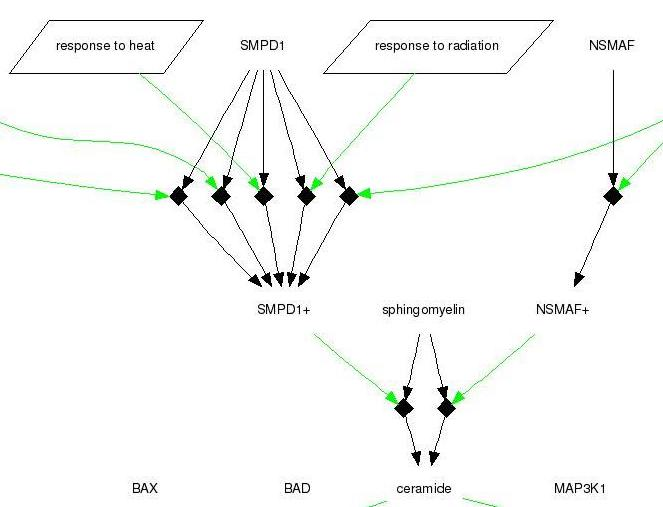
\includegraphics[width=0.8\columnwidth]{CeramidePart.jpg}
\caption{Part of the ceramide signaling pathway imported from BioCarta into the Pathway Interaction Database (PID).
Modifications are drawn with black diamonds.
The entities with a black arrow to the diamond describe the modulation inputs and the entities with an black arrow out of the diamond the modulation output.
The green arrows symbolize positive regulators and the round rectangles complexes.
Pathways are visualized with a trapezium.
The ceramide signaling pathway is one pathway example for providing information which could not be translated to SBML before the creation of the Qualitative Models extension (\qual).
With \qual, it is possible to translate reactions and relations, and to include them in one model.
Even pathway-reaction modulations, like the \lq response to heat\rq{} pathway that positively stimulates the reaction from SMPD1 to SMPD1+, can be described.
(Figure by courtesy of the National Cancer Institute -- http://www.cancer.gov).}
\label{fig:Ceramide}
\end{figure}
%%%%%%%%%%%%%%%%%%%%%%%%%%% END FIGURE 2 %%%%%%%%%%%%%%%%%%%%%%%%%%%%%%%%%%%%%%%%%%%%%%%
%%%%%%%%%%%%%%%%%%%%%%%%%%%%%%%%%%%%%%%%%%%%%%%%%%%%%%%%%%%%%%%%%%%%%%%%%%%%%%%%%%%%%%%%
Finally, the SBML instances are further annotated.
The BioPAX specification allows users to encode arbitrary identifiers for elements.
These can be identifiers for various databases, e.g., UniProt, Entrez Gene, Ensembl, etc.
Unfortunately, the syntax used in BioPAX is sometimes inconsistent, which leads to XML database annotations like ``UniProt'' or ``UniProtKB'' within BioPAX documents that hamper the automatic reading and interpretation of those models by third party applications.


%%%%%%%%%%% Beispiel %%%%%%%%%%%%%%%%%%%%
%  <bp:unificationXref rdf:ID="unificationXref14">
%    <bp:DB rdf:datatype="http://www.w3.org/2001/XMLSchema\#string">UniProt</bp:DB>
%    <bp:ID rdf:datatype="http://www.w3.org/2001/XMLSchema\#string">Q4KMY3</bp:ID>
%  </bp:unificationXref>
%  <bp:unificationXref rdf:ID="unificationXref14">
%    <bp:DB rdf:datatype="http://www.w3.org/2001/XMLSchema\#string">UniProtKB</bp:DB>
%    <bp:ID rdf:datatype="http://www.w3.org/2001/XMLSchema\#string">Q4KMY3</bp:ID>
%  </bp:unificationXref>
%  <bp:unificationXref rdf:ID="unificationXref14">
%    <bp:DB rdf:datatype="http://www.w3.org/2001/XMLSchema\#string">UniProt</bp:DB>
%    <bp:ID rdf:datatype="http://www.w3.org/2001/XMLSchema\#string">Q4KMY3, Q7Z5L2</bp:ID>
%  </bp:unificationXref>
%%%%%%%%%%% Beispiel ENDE %%%%%%%%%%%%%%%%%%%%

In SBML, such identifiers can be expressed as standardized MIRIAM URNs that can be added as annotation to any SBML element.
We support and add MIRIAM identifiers for the following databases: Entrez Gene, Omim, Ensembl, UniProt, ChEBI, DrugBank, Gene Ontology, HGNC, PubChem, 3DMET, NCBI Taxonomy, PDBeChem, GlycomeDB, LipidBank, EC-Numbers (enzyme nomenclature) and various KEGG databases (gene, glycan, reaction, compound, drug, pathway, orthology).
To obtain identifiers for those databases, we map the Entrez Gene identifier, which we annotated on every element in Step 2, to a KEGG identifier.
Using the KEGG API, we then query all of those identifiers to retrieve more descriptive names, descriptions of the elements, and the mentioned database identifiers.
% CW: Entfernt. wurde durch neuen satz (s.o.) ersetzt.
% All supported identifiers from the BioPAX files are parsed, some are manually
% curated by us, and some annotations are supplemented by additional queries to
% the KEGG API for every translated element.
The goal of those annotations is to provide models %that can be used directly by many researchers, no matter what identifiers or databases they use.
whose components can uniquely be identified by any application and be linked to external data sources.
\end{methods}


%%%%%%%%%%%%%%%%%%%%%%%%%%%%%%%%%%%%%%%%%%%%%%%%%%%%%%%%%%%%%%%%%%%%%%%%%%%%%%%%%%%%%%%
%%%%%%%%%%%%%%%%%%%%%%%%%%% TABLE 1 %%%%%%%%%%%%%%%%%%%%%%%%%%%%%%%%%%%%%%%%%%%%%%%%%
\begin{table}[t!h]
\processtable{Description of the translation of BioPAX \Control{}
elements\label{Tab:BioPAX2SBML}} {\begin{tabular}{llll}\toprule
BioPAX            & BioPAX \Controlled              & Converted\\
\Controller       &                                 & SBML \qual\\
                  &                                 & element\\
\midrule
%\textbf{BioPAX Level~3}\\
\multicolumn{3}{c}{\centering \textbf{BioPAX Level~3}}\\
\midrule
PhysicalEntity & BiochemicalReaction                & reaction\\
PhysicalEntity & ComplexAssembly                    & reaction\\
PhysicalEntity & Conversion                         & transition\\
PhysicalEntity & Degradation                        & reaction\\
PhysicalEntity & Transport                          & reaction\\
PhysicalEntity & TransportWithBiochemicalReaction   & reaction\\
PhysicalEntity & Pathway                            & transition\\
PhysicalEntity & TemplateReaction                   & transition\\
\\
Pathway         & BiochemicalReaction               & transition\\
Pathway         & ComplexAssembly                   & transition\\
Pathway         & Conversion                        & transition\\
Pathway         & Degradation                       & transition\\
Pathway         & Pathway                           & transition\\
Pathway         & TemplateReaction                  & transition\\
Pathway         & Transport                         & transition\\
Pathway         & TransportWithBiochemicalReaction  & transition\\
\\\midrule
%\textbf{BioPAX Level~2}\\
\multicolumn{3}{c}{\centering \textbf{BioPAX Level~2}}\\
\midrule
physicalEntity & biochemicalReaction                & reaction\\
physicalEntity & complexAssembly                    & reaction\\
physicalEntity & interaction                        & transition\\
physicalEntity & pathway                            & transition\\
physicalEntity & transport                          & reaction\\
physicalEntity & transportWithBiochemicalReaction   & reaction\\
\\
pathway         & biochemicalReaction               & transition\\
pathway         & complexAssembly                   & transition\\
pathway         & interaction                       & transition\\
pathway         & pathway                           & transition\\
pathway         & transportWithBiochemicalReaction  & transition\\
pathway         & transport                         & transition\\\botrule
\end{tabular}}{BioPAX \Control{} elements consist of a \Controller{} and one
or more \Controlled{} elements.
Depending on the kind of \Controller{} or \Controlled{} element, the \Control{} entity is translated into an SBML reaction or transition.
The table gives an overview of this conversion regarding BioPAX Level~2 and BioPAX Level~3.
}
\end{table}
%%%%%%%%%%%%%%%%%%%%%%%%%%% END TABLE 1 %%%%%%%%%%%%%%%%%%%%%%%%%%%%%%%%%%%%%%%%%%%%%%%



\subsection{Implementation}
The conversion was implemented in Java\texttrademark, using JSBML \citep{Draeger2011} with the Qualitative Models extension, PaxTools \citep{Demir2010}, and the KEGG API \citep{Kanehisa2006}.
PaxTools was used to read the BioPAX files and to manipulate the information content.
With the aid of the KEGG API, this information was extended with MIRIAM identifiers \citep{Novere2005} from the various databases, for instance Entrez Gene, Ensembl, UniProt, etc.



\section{Results and Discussion}
% Aufbau:
% Kern problem: BioPAX-Format der PID Pathways und die fehlende M�glichkeit
% relationen darzustellen.


% 3. Aber das Format ist ungeeignet
% 4. Daher gibt es mehrere Konverter, die folgendes k�nnen reaction
% 5. Das gen�gt nicht weil wir brauchen relationen
% 6. Jetzt gibt es endlich BioPAX to SBML qual, das viel besser ist weil,...
% 7. Im folgenden werden die Merkmale n�her erl�utert.

% 1. PID ist toll weil...
The Pathway Interaction Database (PID) is a curated and peer-reviewed pathway database containing human pathways with molecular signaling and regulatory events provided by the Nature Cancer Institute, BioCarta, and Reactome.
All pathways are provided in XML, BioPAX Level~2, and Level~3 format.

% 2. Man k�nnte so viel tun (Simulation, Informationsverkn\"upfung, tolle SBML programme aufz�hlen?, Siehe KGTrans)
% 3. Aber das Format ist ungeeignet
% 4. Daher gibt es mehrere Konverter, die folgendes k�nnen: reaction
The BioPAX format is perfectly suitable to encode pathway relations and reactions that can be further used for visualization or pathway analysis. However, this format also has its limitations.
Many applications, especially for simulation and modeling of biological networks, use the SBML format \citep{Funahashi2003, Hoops2006}.
Therefore, a few importers and converters for BioPAX into SBML have been developed.
BioPAX \Entity{} elements, which can be genes, proteins, small molecules, etc., can be translated into SBML \species{} and the type of the BioPAX \Entity{} can be encoded as SBO term or MIRIAM annotation of the species itself.
Relations between \Entity{} elements, corresponding to edges in a pathway graph, are also provided with detailed information in BioPAX.
These relations can be transports, biochemical reactions, complex assemblies, etc.
At this point, most translations to SBML usually produce errors or have a massive loss of information because the SBML core specification only provides reactions, which represents real biochemical reactions with substrates, products and enzymes.
Processes, such as modulation of an entity by another one, can not directly be encoded as a reaction, at least not without knowing the exact chemical equation.
Hence, former conversion approaches from BioPAX to SBML did either incorrectly convert those relations to reactions or simply removed them during the translation.
To fill this gap, the SBML community has recently developed the \qual{} specification, which allows users to model arbitrary transitions between species.
%Unfortunately, prior to the creation of the SBML Qualitative Models extension (\qual), it was not possible to properly describe those relations in SBML.
%Hence, the few available converters were either forced to skip the relations, or to create improper pseudo-reactions.

Furthermore, the models themselves just provide the base for further analysis or visualization methods.
Other applications, such as CellDesigner or COPASI, focus on visualization, simulation, analysis, etc. of those models.
Therefore, most of those applications have certain requirements on the models.
For example, to uniquely map mass spectrometry data on a model, it may be required for the model to have UniProt IDs.
To match mRNA expression data or perform gene set enrichment analyses, Entrez Gene identifiers might be required.
Consequently, we provide all annotations that we could gather from the input BioPAX files also in the SBML files and further annotate all \species{} with a plethora of additional identifiers.


% ALTER TEXT:
%Until now, the pathways are not available in SBML format and they can not be translated into SBML without loosing information, because the SBML core specification describes reactions but no other relationships.
%However, the description of those relationships becomes more and more interesting for simulation processes and analysis purposes.
%Many simulation tools use SMBL and not BioPAX, although they can not analyze relations.
%The recently published SBML Qualitative Models extension (\qual) solves this inconvenience and enables the description of such processes in a simple and easily understandable way.

The \qual{} extension has been created recently and, thus, might not be supported by all applications, yet.
Therefore, we decided to build joint SBML core and \qual{} models.
All our SBML files contain a \model{} that corresponds to the SBML core specification, and an additional \qualitativeModel{} that contains all relations.
These models are compatible with older applications, that do not yet support \qual{} but still can read all \species{} and \reactions.
Newer applications that are ready to handle relations can read the additional \qual{} model and process all information that was also available in the BioPAX file.


% Whereas other conversion tools can not translate relations, due to the missing
% SBML specification, we can provide a complete translation of the PID database.
We converted both, the Level~2 and the Level~3 BioPAX files to SBML core, including the \qual{} extension.
The reason for converting both levels was the additional description possibility of gene-regulatory networks and genetic interactions in BioPAX Level~3, which is not supported by Level~2 pathway models.
Since older simulation applications still work with BioPAX Level~2, we also translated these files into SBML in order to prevent loss of information and to be able to use these models, too.
All models are available at \url{http://www.cogsys.cs.uni-tuebingen.de/downloads/Qualitative-Models/}.
Furthermore, we provide our webtool BioPAX2SBML for further BioPAX translations at \url{http://webservices.cs.uni-tuebingen.de/}.


% Kommentiert da info bereits oben erw�hnt wird.
%Since, the models are augmented with additional database information, stored as MIRIAM annotations, the models can easily be used for further simulation purposes. These annotations enable extensive visualization and data exchange between researchers.

\subsection{Comparison to other BioPAX to SBML converters}
%It is difficult to convert BioPAX to SBML \cite{Bauer-Mehren2009}

\newcolumntype{C}{>{\centering\arraybackslash}p{2cm}}
\begin{table*}[htb]
\caption{Comparison of different available converters for KEGG pathways.}
\label{tab:AppVergleich}
%\rowcolors{1}{white}{tableShade2}
\makebox[\textwidth]{
\begin{tabular}{lccc}
\toprule
{\bf }                              & {\bf BioPAX2SBML converter}       & {\bf BiNom}                   & {\bf Sybill} \\
{\bf }                              & {B\"uchel \emph{et al.}}          & {Zinovyev \emph{et al.}}      & {Ruebenacker \emph{et al.}} \\
%{\bf Getestet mit} & PID-BioCarta-ceramide signaling (L2)
%Reacomte-Homarus americanus (L3) & Reactome-Homarus americanus (Level 3) & ceramide signaling von PID-BioCarta \\
{\bf Version}                       & 1.0                               & 2.0                           & 1.0 (Build 119) \\
{\bf Release date}                  & 2012-04-02                        & 2012-04-12                    & 2010-02-11 \\
\midrule
{\bf BioPAX Input Level}            & Level 2 and 3                     & Level 3                       & Level 2 and 3 \\
{\bf SBML  Output Level}            & Level 3 Version 1                 & Level 2 Version 4, Beta       & Level 2 Version 4 \\
                                    & including qual                    & Version for Level 3           &\\
\\
{\bf Signaling support (qual)}      & \checkmark                        & $\times$                      & $\times$  \\
{\bf Valid}                         & \checkmark                        & $\times$                      & $\times$  \\
{\bf Complete}                      & \checkmark                        & \checkmark                    & $\times$  \\
{\bf Robustness}                    & \checkmark                        & \checkmark                    & $\circ$\\
{\bf Machine readable}              & \checkmark                        & \checkmark                    & \checkmark \\
{\bf Human readable}                & \checkmark                        & $\circ$                       & \checkmark \\
\\
{\bf No dublicate entities}         & \checkmark                        & \checkmark                    & \checkmark \\
{\bf Compartements}                 & \checkmark                        & \checkmark                    & \checkmark \\
{\bf Stoichiometry}                 & \checkmark                        & $\times$                      & $\times$ \\
{\bf SBO-terms}                     & \checkmark                        & $\times$                      & $\times$ \\
{\bf Uses appropriate SBO}          & \checkmark                        & $\times$                      & $\times$ \\
{\bf (material entity)}             &                                   &                               & \\
{\bf Xrefs to MIRIAM annotations}   & \checkmark                        & $\times$                      & $\times$ \\
%{\bf Integrate cross refreneces}    & \checkmark                        & $\times$                      & $\times$ \\
{\bf References to original file}   & \checkmark                        & $\times$                      & $\times$ \\
\bottomrule
\end{tabular}
}
{
Sybill (everything is translated to a reaction, there are no reaction modifiers defined), (species are used in reactions, without listing in the species list)
(groups are missing, proteins are missing, links to other pathways are missing)\\
- different entity states are different SBML species, but they are not defined in detail \\
- Wenn kein Pathwayobjekt definiert wurde, wird der pathway nicht �bersetzt \\
%
Binom (order of the reaction lists not correct, some reaction lists are empty, that's ot allowed),
human readable  (abh�nging von der Eingabedatei, keine allgemeinen Regeln) 
}
\end{table*}


\section{Conclusion}
Conversion between different formats is important in all parts of computer science.
In many cases, conversion leads to errors or a loss of information.
The BioPAX to SBML conversion is such an example.
Due to limitations of the SBML core specification, it was not possible to include all relationships between reactive species from BioPAX files in SBML files, while producing correct SBML code.
But with SBML Level~3 Version 1 and the addition of extensions to the specifications, in particular the Qualitative Models extension (\qual), it is now possible to create accurate and specification-conform SBML code.
%, and to minimize or even eliminate the loss of information.
%BioPAX is an RDF format that defines various derived \Entity's which can be genes, proteins, small molecules, etc.
%These can be translated into SBML \species{} and the type of the BioPAX \Entity{} can be encoded as SBO term or MIRIAM annotation of the species itself.
%Relations between \Entity's (which correspond to edges in a pathway graph) are also provided with detailed information in BioPAX.
%These can be transports, biochemical reactions, complex assemblies, etc.
%At this point, most translations to SBML usually produce errors or have a massive loss of information.
%The SBML core specification only provides reactions, which represents real biochemical reactions with substrates, products and enzymes.
%Processes, such as transport mechanisms {\TODO{Gegebenenfalls loeschen}} or modulation of an entity by another one, can not directly be encoded as a reaction, at least not without knowing the exact chemical equation.
%Hence, former conversions approaches from BioPAX to SBML did either incorrectly convert those relations to reactions or simply removed them during the translation.
%To fill this gap, the SBML community has recently developed the \qual{} specification, which allows users to model arbitrary transitions between species.
Using this extension, we produced error-free SBML models while minimizing or even eliminating the loss of information during the translation.

The SBML models, provided along with this publication, consist of SBML \species{} and, wherever possible, exact \reaction{} equations.
All relations from the BioPAX documents that could not be converted to exact reactions have been included as qualitative transitions between qualitative species.
Additional information, such as various identifiers or the type of an entity, are encoded as SBO terms or MIRIAM URNs of the corresponding elements.
%Delete repetition: Furthermore, additional information is added beyond the scope of the BioPAX document by utilizing the KEGG API.
By utilizing the KEGG API it was even possible to complement the translated BioPAX documents with a wealth of information from further databases, such as Entrez Gene, KEGG, etc.

This results in comprehensive and correct SBML models, created for all pathways in the Nature Pathway Interaction Database.
%The files can be downloaded at \url{http://www.cogsys.cs.uni-tuebingen.de/downloads/Qualitative-Models/}.
These models can easily be used, e.g., for further simulation and modeling steps, without having to deal with incorrect input file formats or error-prone conversions.

\section*{Acknowledgements}
%Additional thanks goes to the qualitative models and the JSBML team, which made this work possible.
We wish to acknowledge the Qualitative Models and JSBML teams.
% Special thanks should be given to ...
% I wish to acknowledge

\paragraph{Funding\textcolon}
Federal Ministry of Education and Research (BMBF, Germany) in the National
Genome Research Network (NGFN+) under grant number 01GS08134 and Virtual Liver
Network under grant number 0315756.
\paragraph{Conflict of interest\textcolon} None declared.


\bibliographystyle{natbib}
%\bibliographystyle{achemnat}
%\bibliographystyle{plainnat}
%\bibliographystyle{abbrv}
%\bibliographystyle{bioinformatics}
%\bibliographystyle{plain}
%
\bibliography{document}

% Bauer-Mehren is missing
%\begin{thebibliography}{}
%
%\bibitem[Berenguier {\em et~al.}(2011)Berenguier, Chaouiya, Naldi, Thieffry,
%  and van Iersel]{QualSpecification}
%Berenguier, D., Chaouiya, C., Naldi, A., Thieffry, D., and van Iersel, M.~P.
%  (2011).
%\newblock {Qualitative Models} (qual).
%\newblock Specification available at
%  \url{http://sbml.org/Community/Wiki/SBML\_Level\_3\_Proposals/Qualitative\_Models}.
%  Accessed 2012 Mar 22.
%
%\bibitem[Courtot {\em et~al.}(2011)Courtot, Juty, Kn\"{u}pfer, Waltemath,
%  Zhukova, Dr\"{a}ger, Dumontier, Finney, Golebiewski, Hastings, Hoops,
%  Keating, Kell, Kerrien, Lawson, Lister, Lu, Machne, Mendes, Pocock,
%  Rodriguez, Villeger, Wilkinson, Wimalaratne, Laibe, Hucka, and
%  Nov\`{e}re]{SBO}
%Courtot, M., Juty, N., Kn\"{u}pfer, C. {\em et~al.} (2011).
%\newblock Controlled vocabularies and semantics in systems biology.
%\newblock {\em Mol Syst Biol\/}, {\bf 7}, 543.
%
%\bibitem[Demir {\em et~al.}(2010)Demir, Cary, Paley, Fukuda, Lemer, Vastrik,
%  Wu, D'Eustachio, Schaefer, Luciano, Schacherer, Martinez-Flores, Hu,
%  Jimenez-Jacinto, Joshi-Tope, Kandasamy, Lopez-Fuentes, Mi, Pichler,
%  Rodchenkov, Splendiani, Tkachev, Zucker, Gopinath, Rajasimha, Ramakrishnan,
%  Shah, Syed, Anwar, Babur, Blinov, Brauner, Corwin, Donaldson, Gibbons,
%  Goldberg, Hornbeck, Luna, Murray-Rust, Neumann, Reubenacker, Samwald, van
%  Iersel, Wimalaratne, Allen, Braun, Whirl-Carrillo, Cheung, Dahlquist, Finney,
%  Gillespie, Glass, Gong, Haw, Honig, Hubaut, Kane, Krupa, Kutmon, Leonard,
%  Marks, Merberg, Petri, Pico, Ravenscroft, Ren, Shah, Sunshine, Tang, Whaley,
%  Letovksy, Buetow, Rzhetsky, Schachter, Sobral, Dogrusoz, McWeeney, Aladjem,
%  Birney, Collado-Vides, Goto, Hucka, Nov\`{e}re, Maltsev, Pandey, Thomas,
%  Wingender, Karp, Sander, and Bader]{Demir2010}
%Demir, E., Cary, M.~P., Paley, S. {\em et~al.} (2010).
%\newblock The {BioPAX} community standard for pathway data sharing.
%\newblock {\em Nat Biotechnol\/}, {\bf 28}(9), 935--942.
%
%\bibitem[Dr\"ager {\em et~al.}(2011)Dr\"ager, Rodriguez, Dumousseau, D\"orr,
%  Wrzodek, Le~Nov\`{e}re, Zell, and Hucka]{Draeger2011}
%Dr\"ager, A., Rodriguez, N., Dumousseau, M., D\"orr, A., Wrzodek, C.,
%  Le~Nov\`{e}re, N., Zell, A., and Hucka, M. (2011).
%\newblock {JSBML: a flexible Java library for working with SBML}.
%\newblock {\em Bioinformatics\/}, {\bf 27}(15), 2167--2168.
%
%\bibitem[{European Bioinformatics Institute -- Computational Systems
%  Neurobiology Group}(2011){European Bioinformatics Institute -- Computational
%  Systems Neurobiology Group}]{SBFC}
%{European Bioinformatics Institute -- Computational Systems Neurobiology Group}
%  (2011).
%\newblock {System Biology Format Converter (SBFC)}.
%\newblock Software available from
%  \url{http://www.ebi.ac.uk/compneur-srv/sbml/converters/SBMLtoBioPAX.html}.
%  Accessed 2012 Mar 22.
%
%\bibitem[Funahashi {\em et~al.}(2007)Funahashi, Jouraku, Matsuoka, and
%  Kitano]{Funahashi2007}
%Funahashi, A., Jouraku, A., Matsuoka, Y., and Kitano, H. (2007).
%\newblock {Integration of CellDesigner and SABIO-RK.}
%\newblock {\em In Silico Biol\/}, {\bf 7}(2 Suppl), S81--S90.
%
%\bibitem[Hucka {\em et~al.}(2003)Hucka, Finney, Sauro, Bolouri, Doyle, Kitano,
%  Arkin, Bornstein, Bray, Cornish-Bowden, Cuellar, Dronov, Gilles, Ginkel, Gor,
%  Goryanin, Hedley, Hodgman, Hofmeyr, Hunter, Juty, Kasberger, Kremling,
%  Kummer, Nov\`{e}re, Loew, Lucio, Mendes, Minch, Mjolsness, Nakayama, Nelson,
%  Nielsen, Sakurada, Schaff, Shapiro, Shimizu, Spence, Stelling, Takahashi,
%  Tomita, Wagner, Wang, and Forum]{Hucka2003}
%Hucka, M., Finney, A., Sauro, H.~M. {\em et~al.} (2003).
%\newblock {The systems biology markup language (SBML): a medium for
%  representation and exchange of biochemical network models.}
%\newblock {\em Bioinformatics\/}, {\bf 19}(4), 524--531.
%
%\bibitem[Kanehisa {\em et~al.}(2006)Kanehisa, Goto, Hattori, Aoki-Kinoshita,
%  Itoh, Kawashima, Katayama, Araki, and Hirakawa]{Kanehisa2006}
%Kanehisa, M., Goto, S., Hattori, M. {\em et~al.} (2006).
%\newblock From genomics to chemical genomics: new developments in {KEGG}.
%\newblock {\em Nucleic Acids Res\/}, {\bf 34}(Database issue), D354--D357.
%
%\bibitem[Mi {\em et~al.}(2011)Mi, Muruganujan, Demir, Matsuoka, Funahashi,
%  Kitano, and Thomas]{Mi2011}
%Mi, H., Muruganujan, A., Demir, E., Matsuoka, Y., Funahashi, A., Kitano, H.,
%  and Thomas, P.~D. (2011).
%\newblock {BioPAX support in CellDesigner.}
%\newblock {\em Bioinformatics\/}, {\bf 27}(24), 3437--3438.
%
%\bibitem[Le~Nov\`{e}re {\em et~al.}(2005)Le~Nov\`{e}re, Finney, Hucka, Bhalla,
%  Campagne, Collado-Vides, Crampin, Halstead, Klipp, Mendes, Nielsen, Sauro,
%  Shapiro, Snoep, Spence, and Wanner]{Novere2005}
%Le~Nov\`{e}re, N., Finney, A., Hucka, M. {\em et~al.} (2005).
%\newblock Minimum information requested in the annotation of biochemical models
%  {(MIRIAM)}.
%\newblock {\em Nat Biotechnol\/}, {\bf 23}(12), 1509--1515.
%
%\bibitem[R\"ubenacker {\em et~al.}(2009)R\"ubenacker, Moraru, Schaff, and
%  Blinov]{Ruebenacker2009}
%R\"ubenacker, O., Moraru, I.~I., Schaff, J.~C., and Blinov, M.~L. (2009).
%\newblock {Integrating BioPAX pathway knowledge with SBML models.}
%\newblock {\em IET Syst Biol\/}, {\bf 3}(5), 317--328.
%
%\bibitem[Schaefer {\em et~al.}(2009)Schaefer, Anthony, Krupa, Buchoff, Day,
%  Hannay, and Buetow]{Schaefer2009}
%Schaefer, C.~F., Anthony, K., Krupa, S. {\em et~al.} (2009).
%\newblock {PID: the Pathway Interaction Database.}
%\newblock {\em Nucleic Acids Res\/}, {\bf 37}(Database issue), D674--D679.
%
%\bibitem[Smoot {\em et~al.}(2011)Smoot, Ono, Ruscheinski, Wang, and
%  Ideker]{Smoot2011a}
%Smoot, M.~E., Ono, K., Ruscheinski, J., Wang, P.-L., and Ideker, T. (2011).
%\newblock Cytoscape 2.8: new features for data integration and network
%  visualization.
%\newblock {\em Bioinformatics\/}, {\bf 27}(3), 431--432.
%
%\bibitem[Zinovyev {\em et~al.}(2008)Zinovyev, Viara, Calzone, and
%  Barillot]{Zinovyev2008}
%Zinovyev, A., Viara, E., Calzone, L., and Barillot, E. (2008).
%\newblock {BiNoM: a Cytoscape plugin for manipulating and analyzing biological
%  networks.}
%\newblock {\em Bioinformatics\/}, {\bf 24}(6), 876--877.
%
%\bibitem[Funahashi {\em et~al.}(2003)Funahashi, Morohashi, Kitano, and
%  Tanimura]{Funahashi2003}
%Funahashi, A., Morohashi, M., Kitano, H., and Tanimura, N. (2003).
%\newblock {CellDesigner: a process diagram editor for gene-regulatory and biochemical networks.}
%\newblock {\em BIOSILICO\/}, {\bf 1}(5), 159--162.
%
%\bibitem[Zinovyev {\em et~al.}(2006)Hoops, Sahle, Gauges, Lee, Pahle,
%  Simus, Singhal, Xu, Mendes, and Kummer]{Hoops2006}
%Hoops, S., Sahle, S., Gauges, R. {\em et~al.} (2006).
%\newblock {COPASI--a COmplex PAthway SImulator.}
%\newblock {\em Bioinformatics\/}, {\bf 22}(24), 3067--3074.
%
%
%\end{thebibliography}


\end{document}
